\section{Einführung}\script{3}
Signale lassen sich in 3 Klassen oder keine davon einteilen. Alle beschränkten Signale endlicher Dauer, die auf einem endlichen Zeitintervall von Null verschieden sind, sind stets Energiesignale und gehören zur Klasse 1. \\

\begin{itemize}[nosep]
	\item Klasse 1 $\rightarrow$ Energiesignale
	\item Klasse 2a $\rightarrow$ Leistungssignal periodisch
	\item Klasse 2b $\rightarrow$ Leistungssignal aperiodisch
\end{itemize} 

\begin{center}
	\rotatebox{90}{
		\bgroup
		\def\arraystretch{2.5}
		\begin{tabular}{p{2cm}|C{3cm}|C{6cm}}
			& Klasse 1 & Klasse 2 \\ \toprule
			& 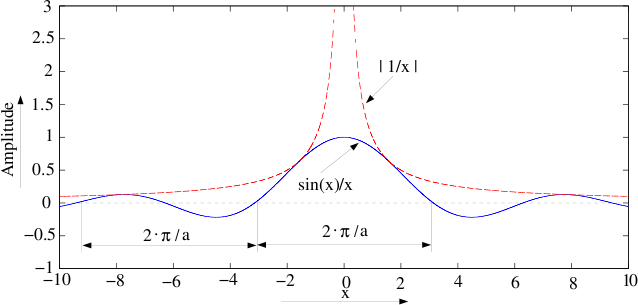
\includegraphics[width=0.3\columnwidth]{Images/einergiesignal} & 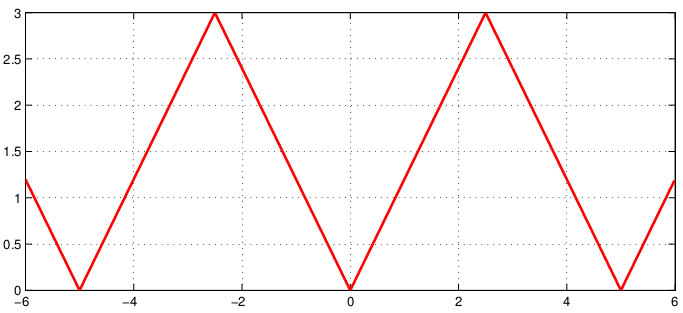
\includegraphics[width=0.3\columnwidth]{Images/leistungssignal_2a} 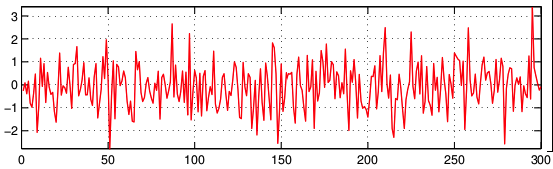
\includegraphics[width=0.3\columnwidth]{Images/leistungssignal_2b} \\ \midrule
			
			Signal-\textbf{leistung} $P$ & $0$ & $\frac{1}{T}\lim\limits_{T\rightarrow\infty}\int\limits_{-T/2}^{T/2} \left|f(t)\right|^2dt $ \\ \midrule
			Signal-\textbf{energie} $W$ & $\lim\limits_{T\rightarrow\infty}\int\limits_{-T/2}^{T/2} \left|f(t)\right|^2dt $ & $\infty$
			
		\end{tabular}
		\egroup
}
\end{center}



\subsection{Mittelwerte}

\noindent 
Linearer Mittelwert (Signal Klasse 2a): \[\overline{X} = X_0 = \frac{1}{T}\int\limits_{-T/2}^{T/2}x(t)dt\]
Quadratischer Mittelwert (Signal Klasse 2a) \textbf{Leistung}: \[X^2 =  \frac{1}{T}\int\limits_{-T/2}^{+T/2}\left|x(t)\right|^2dt\] 
Effektivwert (RMS): \[X_{eff} = X_{rms} = \sqrt{X^2}\] 
Varianz: \[ \var(x) =  \sigma^2 = \frac{1}{T}\int\limits_{-T/2}^{+T/2}(x(t) - \overline{X})^2dt \]
Standardabweichung: \[ \sigma = \sqrt{Var(x)}\]
Gleichung: 
\[X^2 = \var(|x|) + |\overline{X}|^2\]

\subsection{Funktionen}
\subsubsection{Autokorrelationsfunktion (AKF)}\script{8}
AFK $\varphi_{xx}(\tau)$ ist ein Mass für die innere \textbf{Kohärenz} (Ähnlichkeit) eines Signals und beschreibt wie weit zeitliche verschobene Signalteile zusammenhängen.

Klasse 1:
\begin{align*}
	\varphi_{xx}(\tau) &= \lim\limits_{T\rightarrow\infty}\int\limits_{-T/2}^{T/2}x(t)x(t-\tau)dt \\
	&= \lim\limits_{T\rightarrow\infty}\int\limits_{-T/2}^{T/2}x(t+\tau)x(t)dt
\end{align*}

Klasse 2:
\begin{align*}
	\varphi_{xx}(\tau) &= \lim\limits_{T\rightarrow\infty}\frac{1}{T}\int\limits_{-T/2}^{T/2}x(t)x(t-\tau)dt \\
	&= \lim\limits_{T\rightarrow\infty}\frac{1}{T}\int\limits_{-T/2}^{T/2}x(t+\tau)x(t)dt
\end{align*}

\noindent\textbf{Eigenschaften}:
\begin{itemize}[nosep]
	\item $\varphi_{xx}(\tau) = \varphi_{xx}(-\tau)$ ist eine gerade Funktion
	\item $P = \varphi_{xx}(\tau = 0) = X_0^2 + \sigma^2$ Diracstoss bei $\tau =0$ entspricht der Leistung des Signals 
	\item $\varphi_{xx}(\tau) = \varphi_{xx}(\tau \pm kT)$ ist periodisch mit gleicher Periode wie Signal $x(t)$
\end{itemize}

~\\

\noindent\textbf{Beispiel:}\\
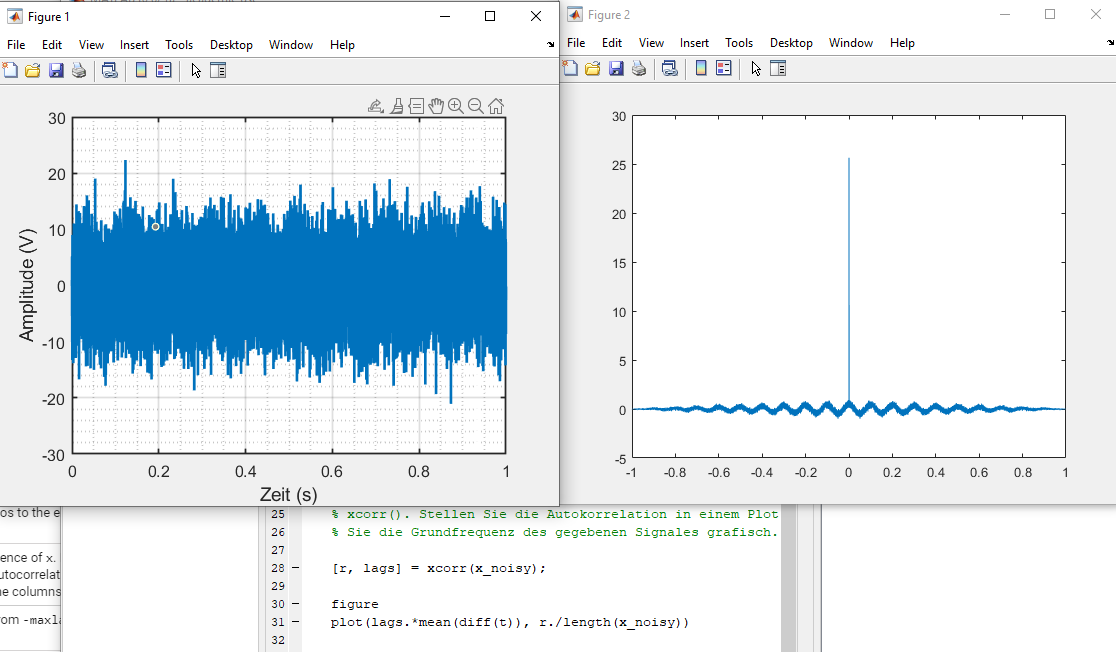
\includegraphics[width=\linewidth]{Images/akf_example}

\subsubsection{Kreuzkorrelationsfunktion (KKF)}\script{11}
KKF sagt wie ähnlich sind zwei verschiedene Signale sind. Die KKF ist nicht \textbf{zwingend} Symmetrisch und $\max$ ist auch nicht bei $\varphi_{x_1x_2}(0)$.

Klasse 1:
\begin{align*}
	\varphi_{x_1x_2}(\tau) &= \lim\limits_{T\rightarrow\infty}\int\limits_{-T/2}^{T/2}x_1(t)x_2(t-\tau)dt \\
	&= \lim\limits_{T\rightarrow\infty}\int\limits_{-T/2}^{T/2}x_1(t)x_2(t+\tau)dt
\end{align*}

Klasse 2:
\begin{align*}
	\varphi_{x_1x_2}(\tau) &= \lim\limits_{T\rightarrow\infty}\frac{1}{T}\int\limits_{-T/2}^{T/2}x_1(t)x_2(t-\tau)dt \\
	&= \lim\limits_{T\rightarrow\infty}\frac{1}{T}\int\limits_{-T/2}^{T/2}x_1(t)x_2(t+\tau)dt
\end{align*}

\subsubsection{Faltung}
Die Faltung ist eine lineare Operation von zwei Signalen und wird auch convolution gennant \script{14}.
\[
y(t) = \int\limits_{-\infty}^{\infty}f(\tau)g(t - \tau)d\tau = f(t) * g(t)
\]
Tips zur visuellen Faltung: Rechte Funktion $g$ an y-Achse spiegeln und dann verschieben von links nach Rechts. Zu jedem Zeitpunkt ist die Fläche der überlappung mit $f$ der Ausgang $y$
	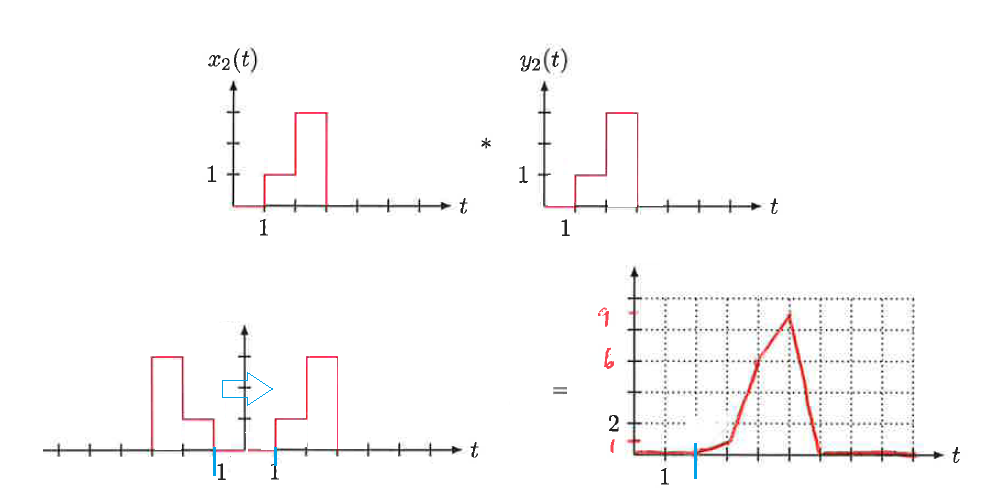
\includegraphics[width=\linewidth,keepaspectratio=true]{Images/faltung}

\noindent\textbf{Maximum einer Faltung}
Das Maximum der Faltung ist erreicht, wenn sich die Flächen maximal schneiden.
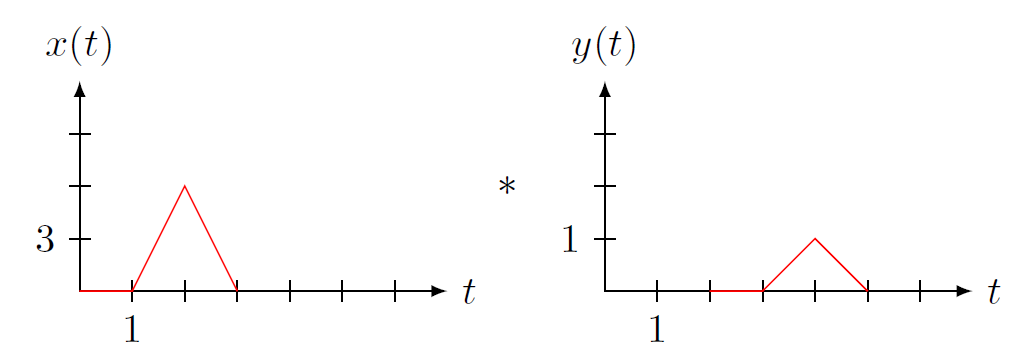
\includegraphics[width=\columnwidth]{Images/faltung_maxi}
\[
\max = 2\cdot \int_{0}^{1}6x \cdot x \cdot dx = \left.12\frac{x^3}{3}\right|_0^1 = 4
\]


\subsubsection{Sprungfunktion $u(t)$}\script{17}
\begin{center}
	\begin{minipage}{0.2\textwidth}
		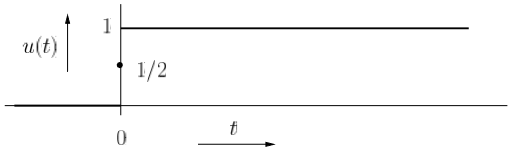
\includegraphics[width=\linewidth,keepaspectratio=true]{Images/sprungfunktion}
	\end{minipage}%%% to prevent a space
	\begin{minipage}{0.2\textwidth}
		\[u(t) = \begin{cases*}
			0 & \text{für } t $\lt$ 0 \\
			\frac{1}{2} & \text{für } t = 0 \\
			1 &\text{für } t $\gt$ 0 \\
		\end{cases*}\]
	\end{minipage}
\end{center}

\subsubsection{Signumfunktion $\sgn(t)$}\script{17}
\subsubsection{Rechteckimpuls $p_a(t)$}\script{19}
\subsubsection{Dreickimpuls $\Lambda_a(t)$}\script{20}
\subsubsection{Sincfunktion $\sinc(t)$}\script{20}
\begin{center}
	\begin{minipage}{0.2\textwidth}
		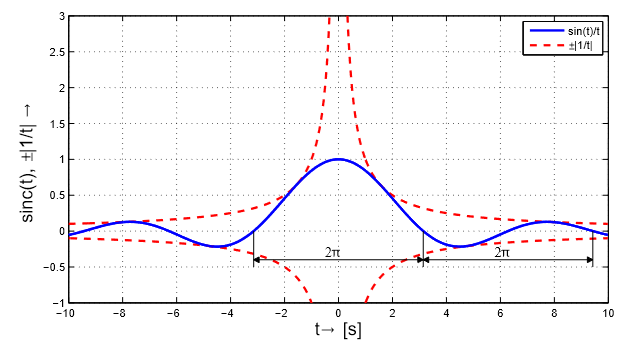
\includegraphics[width=\linewidth,keepaspectratio=true]{Images/sinc}
	\end{minipage}%%% to prevent a space
	\begin{minipage}{0.2\textwidth}
		\[\sinc(t) = \frac{\sin(t)}{t}\]
	\end{minipage}
\end{center}

\subsubsection{Delta-Funktion}\script{21}
\begin{center}
	\begin{minipage}{0.2\textwidth}
		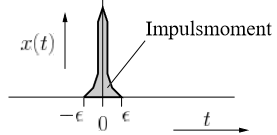
\includegraphics[width=\linewidth,keepaspectratio=true]{Images/dirac}
	\end{minipage}%%% to prevent a space
	\begin{minipage}{0.2\textwidth}
		\[\delta(t) = \begin{cases*}
			\infty & \text{für } t = 0 \\
			0 & \text{sonst}
		\end{cases*}\]
	\end{minipage}
\end{center}

\textbf{Eigenschaften}\\
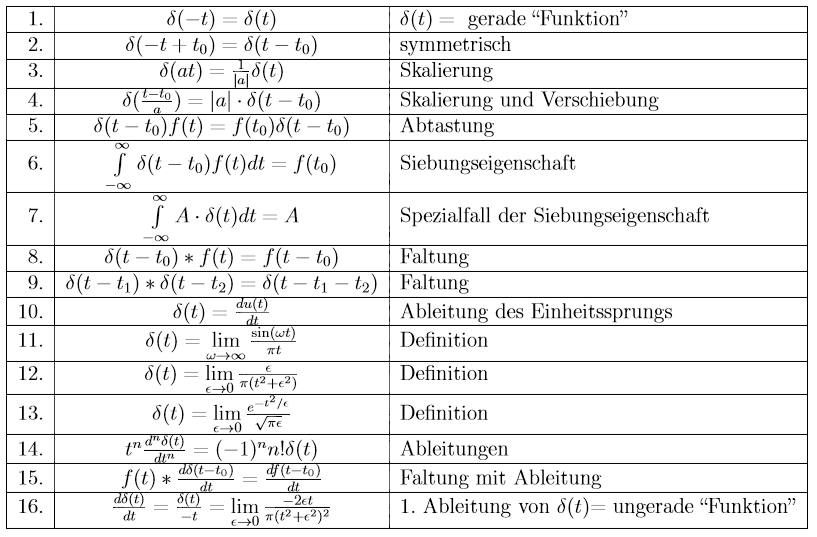
\includegraphics[width=\columnwidth]{Images/delta}

\subsection{Amplitudentdichte}\script{28}
Die Amplitudendichte $p(a)$ ist ein Mass für die relative Zeit ( Zeit /
Gesamtzeit = Wahrscheinlichkeit), während der sich das Signal in einem
bestimmten Amplitudenintervall $\frac{a\pm da}{2}$ aufhält. \textit{Zeit während
sich Signal in bestimmtem Amplitudenintervall aufhält}
\[
p(a) = \lim\limits_{da\rightarrow 0}\frac{\sum t\overbrace{\left(a - \frac{da}{2} < x(t) \leq a + \frac{da}{2}\right)}^{dt}}{T\cdot da} = \frac{1}{T} \cdot \frac{dt}{da}
\]
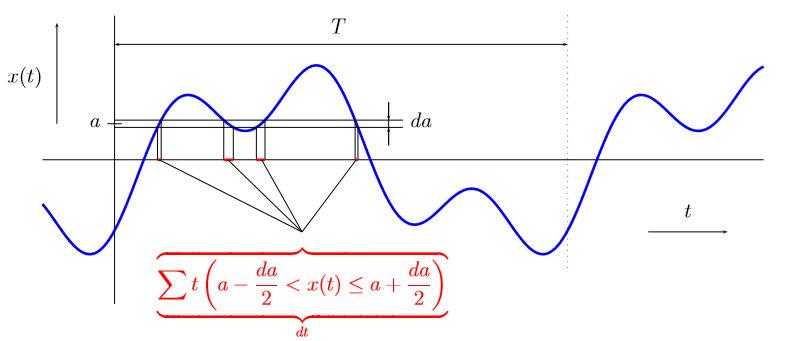
\includegraphics[width=\columnwidth]{Images/aplitudenspektrum}

Dabei ergibt sich eine Wahrscheinlichkeitsdichte $p(a)$ welche immer $\int_{-\infty}^{\infty}p(a)da = 1$ hat! Zudem hat die Aplitudendichte new negative Werte
~\\ ~\\
\textbf{Wichtig:} Siehe auch \script{38} für weitere Wahrscheinlichkeitsdichten für stochastische Signale.

\subsection{Rauschen}\script{25}
Wenn die Frequenzaanteile von einem Rauschen normalverteilt sind, spricht man von einem \textbf{weissen Rauschen}. 
Rauschen in Widerständen sind Temperatur $T$ in abs. Kelvin, Frequenz $\Delta f$ und Boltzmann-Konstante $k = 1.38\cdot10^{-23}\frac{J}{K}$ und Widerstand $R$ abhängig.

\noindent \textbf{Effektive Rauschleistung:}
\[
P_r = k\cdot T\cdot \Delta f
\]

\noindent \textbf{Effektive Rauschspannung:}
\[
U_r = \sqrt{4\cdot k\cdot T\cdot \Delta f \cdot R}
\]

\subsubsection{SNR}
Zur Qualitätsbewertung von Signalen wird das Verhältnis zwischen \textbf{Nutzleistung} $P_s$ und \textbf{Rauschleistung} $P_r$ gebildet. Dieses Signal-to-noise Ratio (SNR) wird \textbf{Störabstand} $a_r$ genannt:
\[
a_r = 10\cdot \log_{10}\left(\frac{P_s}{P_r}\right) = 20\cdot \log_{10}\left(\frac{U_s}{U_r}\right)
\]

\subsubsection{Rausch-Addition}
Die Summe der Signale addieren auch das Rauschen. Diese können durch die Faltung der Wahrscheinlichkeitsdichten berechnet werden.

\[
p(a) = \int_{-\infty}^{\infty}p_1(x_1)*p_2(\underbrace{a - x_1}_{x_2})dx_1
\]

\begin{center}
	\noindent 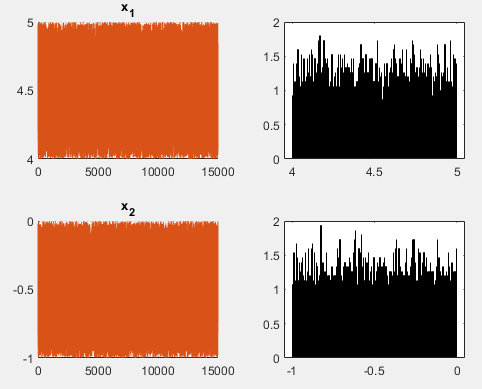
\includegraphics[width=0.7\columnwidth]{Images/rauschen_example1}
\noindent 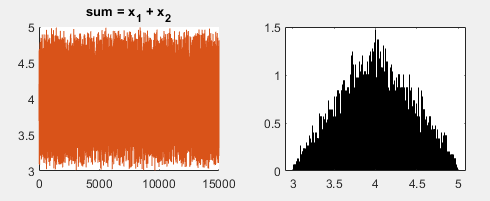
\includegraphics[width=0.7\columnwidth]{Images/rauschen_example2}
\end{center}


